
\section{Functional Specification}

This section provides a comprehensive overview of the system's functionality. It includes a use case diagram illustrating the system's interactions and a detailed textual description of each use case.

\subsection{Use Case Diagram}

Figure \ref{fig:Sprint 1 Use Case Diagram} offers us an overview by presenting a visual description of the functional
behaviour of our tool during the first sprint. This diagram sums up the interactions among the actors and the
diverse use cases within the system.

\begin{figure}[ht]
	\centering
	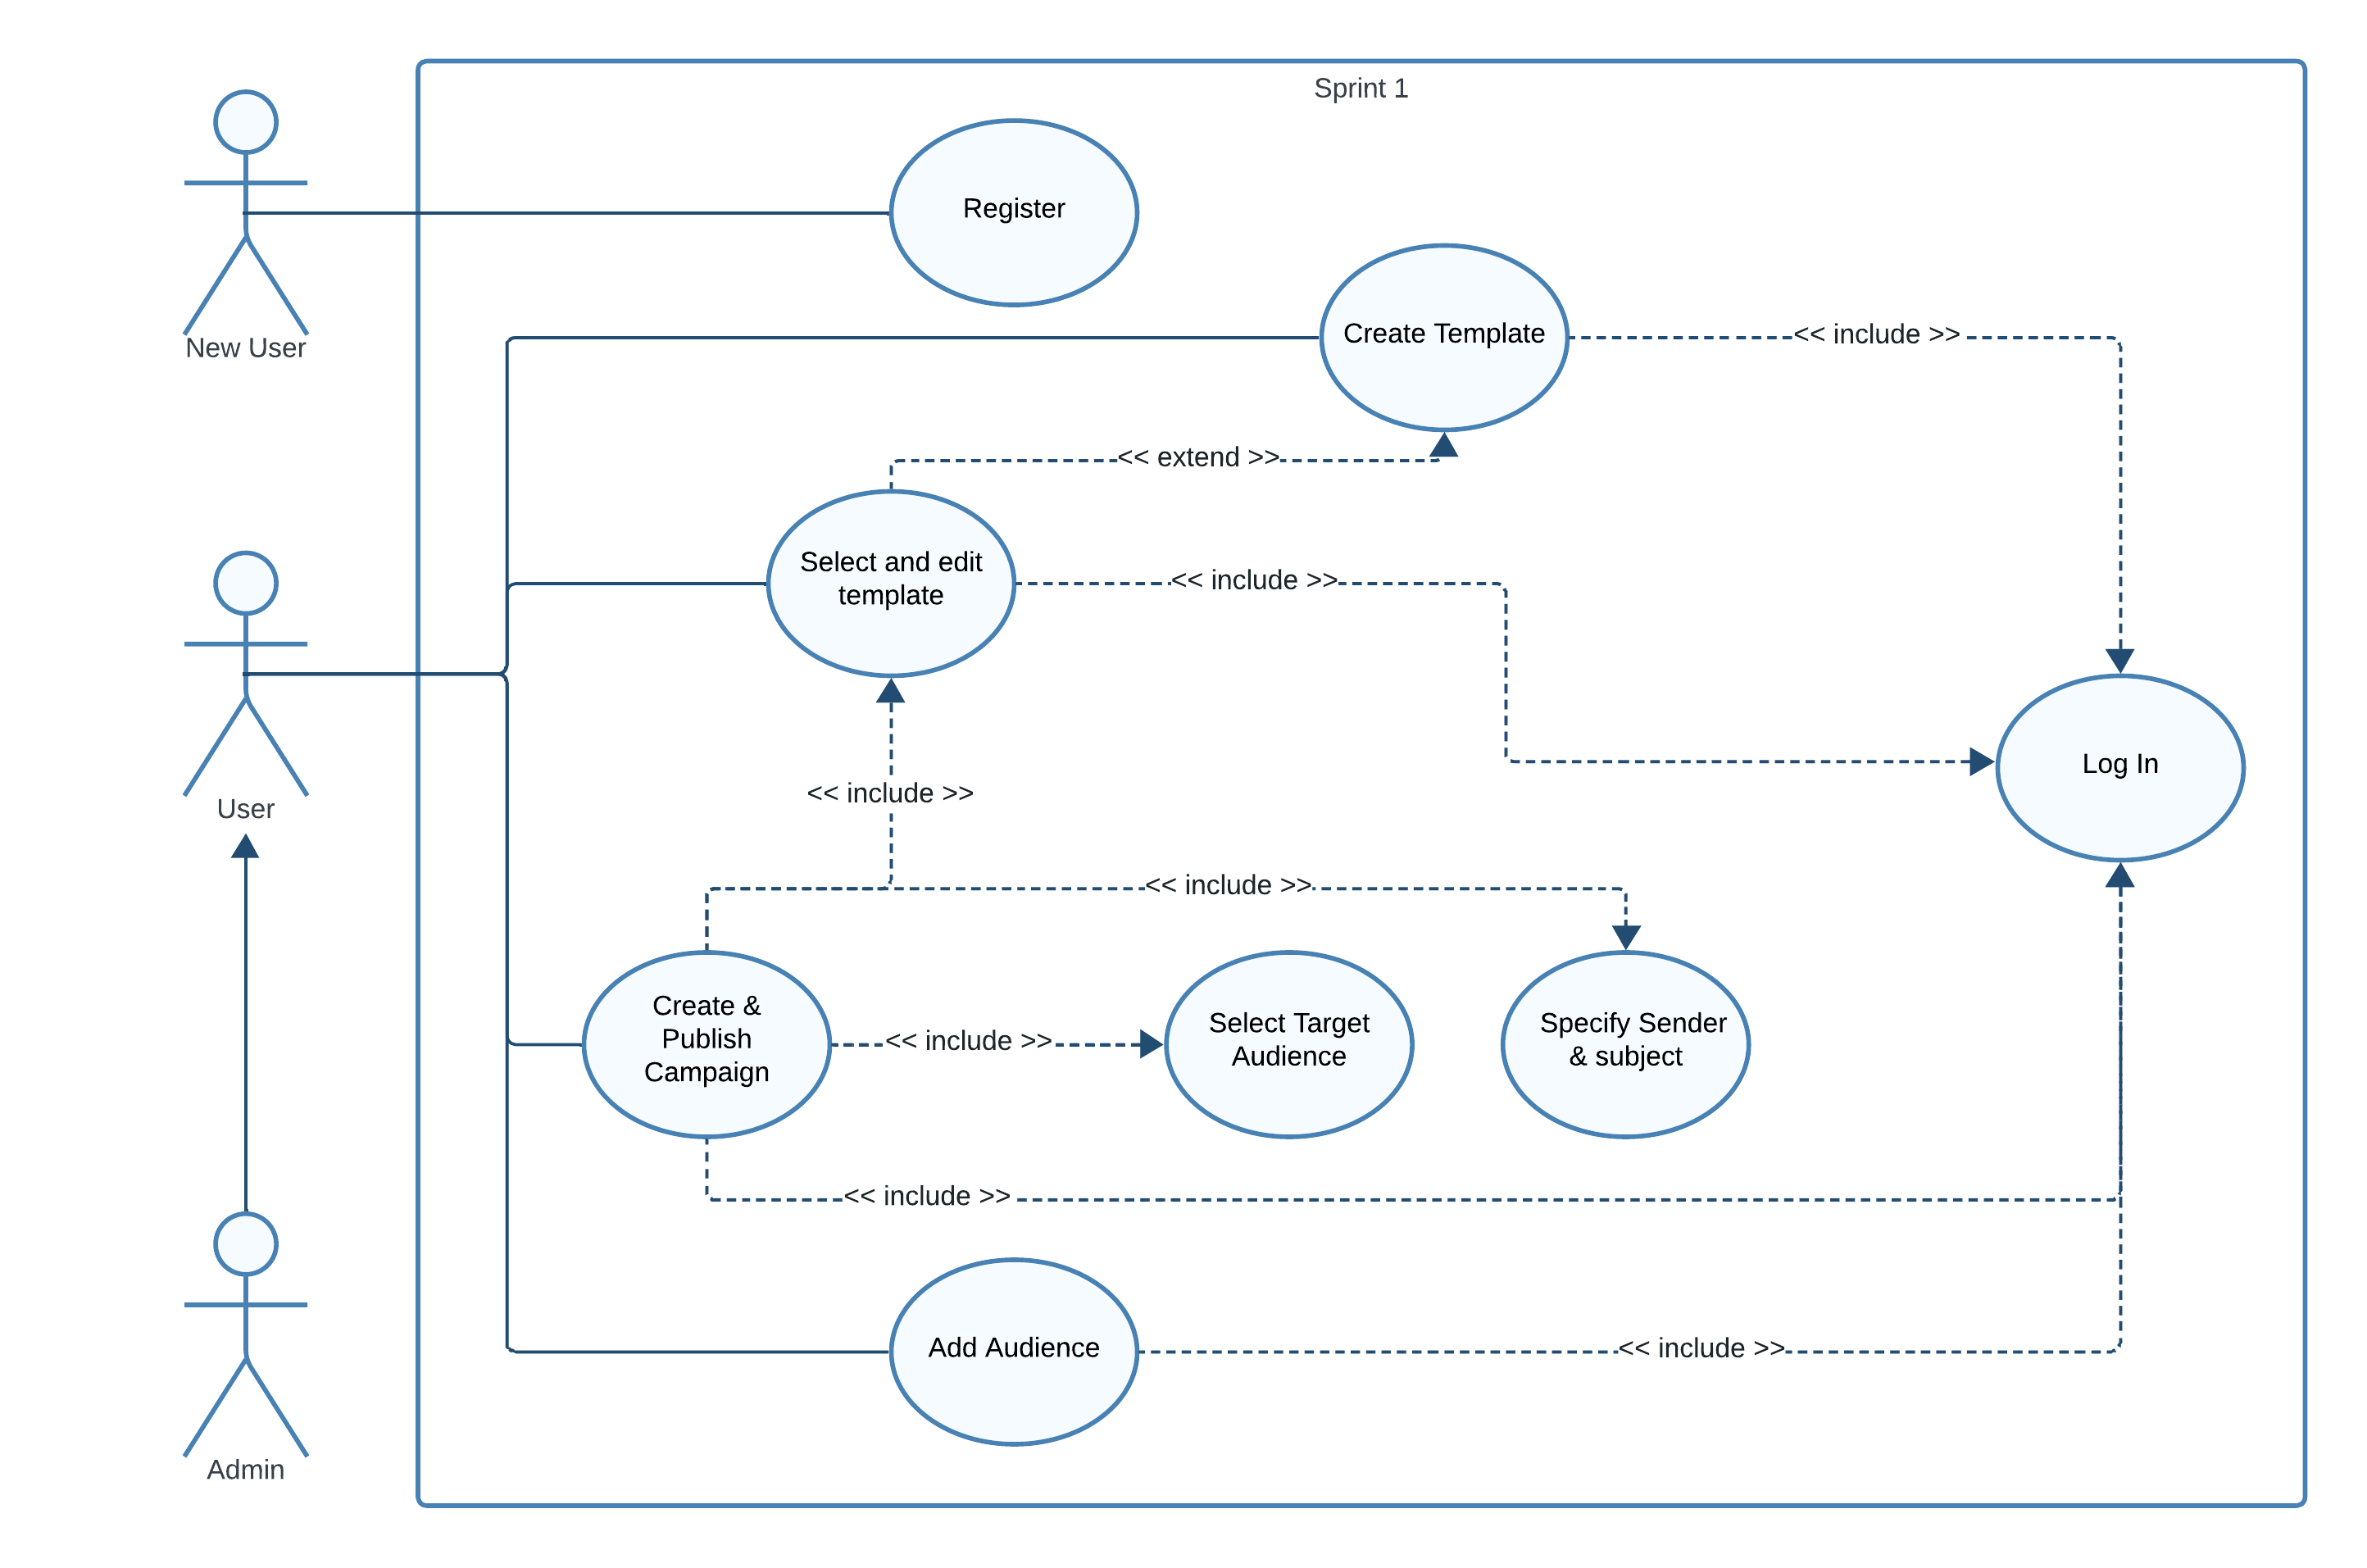
\includegraphics[width=\linewidth]{Images/Sprint1/use_case_diag_sprint_1.png}
	\caption{Sprint 1 Use Case Diagram}
	\label{fig:Sprint 1 Use Case Diagram}
\end{figure}

\subsection{Textual Description of Use Cases}

The following tables provide a detailed description of the use cases. This includes the actor, the goal of the use case, the preconditions, the basic flow, the alternative flows, and the postconditions.

\subsubsection{Use Case 1: Register}

Table \ref{tab:Use Case 1 Register} presents a textual description of a use case: Register.

\begin{table}[ht]
	\centering
	\begin{tabularx}{\textwidth}{|l|X|}
		\hline
		\textbf{Actor}             & New User                                                              \\
		\hline
		\textbf{Goal}              & To register a new user to the system                                  \\
		\hline
		\textbf{Preconditions}     & The new user has accessed the registration page                       \\
		\hline
		\textbf{Basic Flow}        & 1. The new user enters their details in the registration form         \\
		                           & 2. The system validates the entered details                           \\
		                           & 3. The system creates a new user account                              \\
		\hline
		\textbf{Alternative Flows} & If the entered details are invalid, the system shows an error message \\
		\hline
		\textbf{Postconditions}    & A new user account is created and the new user can log in             \\
		\hline
	\end{tabularx}
	\caption{Use Case 1: Register}
	\label{tab:Use Case 1 Register}
\end{table}

\subsubsection{Use Case 2: Log In}

Table \ref{tab:Use Case 2 Authenticate} presents a textual description of a use case: Log In.

\begin{table}[ht]
	\centering
	\begin{tabularx}{\textwidth}{|l|X|}
		\hline
		\textbf{Actor}             & User, Admin                                                               \\
		\hline
		\textbf{Goal}              & To authenticate a user to the system                                      \\
		\hline
		\textbf{Preconditions}     & The user has a registered account and has accessed the login page         \\
		\hline
		\textbf{Basic Flow}        & 1. The user enters their login credentials                                \\
		                           & 2. The system validates the entered credentials                           \\
		                           & 3. The system logs the user in                                            \\
		\hline
		\textbf{Alternative Flows} & If the entered credentials are invalid, the system shows an error message \\
		\hline
		\textbf{Postconditions}    & The user is authenticated and logged in to the system                     \\
		\hline
	\end{tabularx}
	\caption{Use Case 2: Authenticate}
	\label{tab:Use Case 2 Authenticate}
\end{table}

\subsubsection{Use Case 3: Create Email Template}

Table \ref{tab:Use Case 3 Create Email Template} presents a textual description of a use case: Create Email Template.

\begin{table}[ht]
	\centering
	\begin{tabularx}{\textwidth}{|l|X|}
		\hline
		\textbf{Actor}             & User, Admin                                                  \\
		\hline
		\textbf{Goal}              & To create a new email template                               \\
		\hline
		\textbf{Preconditions}     & The user is authenticated and has accessed the email builder \\
		\hline
		\textbf{Basic Flow}        & 1. The user selects the option to create a new template      \\
		                           & 2. The user designs the template and saves it                \\
		\hline
		\textbf{Alternative Flows} & None                                                         \\
		\hline
		\textbf{Postconditions}    & A new email template is created and saved in the system      \\
		\hline
	\end{tabularx}
	\caption{Use Case 3: Create Email Template}
	\label{tab:Use Case 3 Create Email Template}
\end{table}


\subsubsection{Use Case 4: Create Campaign}

Table \ref{tab:Use Case 4 Create Campaign} presents a textual description of a use case: Create Campaign.

\begin{table}[ht]
	\centering
	\begin{tabularx}{\textwidth}{|l|X|}
		\hline
		\textbf{Actor}             & User, Admin                                                                                             \\
		\hline
		\textbf{Goal}              & To Create and publish a campaign                                                                        \\
		\hline
		\textbf{Preconditions}     & The user is authenticated, has selected an email template, and has specified the recipient, the sender  \\
		\hline
		\textbf{Basic Flow}        & 1. The user clicks the "save and publish" button                                                        \\
		                           & 2. The system sends the email to the specified recipient                                                \\
		                           & 3. The system saves the published campaign                                                              \\
		\hline
		\textbf{Alternative Flows} & If the recipients or the sender emails are not real or do not exist, the system should notify the user. \\
		\hline
		\textbf{Postconditions}    & The email has been sent to the specified recipient and the campaign has been saved.                     \\
		\hline
	\end{tabularx}
	\caption{Use Case 4: Create Campaign}
	\label{tab:Use Case 4 Create Campaign}
\end{table}



\subsubsection{Use Case 5: Create Audeience}

Table \ref{tab:Use Case 5 Create Audience} presents a textual description of a use case: Create Audience.

\begin{table}[ht]
	\centering
	\begin{tabularx}{\textwidth}{|l|X|}
		\hline
		\textbf{Actor}             & User, Admin                                                        \\
		\hline
		\textbf{Goal}              & To Create and publish a campaign                                   \\
		\hline
		\textbf{Preconditions}     & The user is authenticated                                          \\
		\hline
		\textbf{Basic Flow}        & 1. The user fills the necessairy fields                            \\
		                           & 2. The system validates the entered details and saves the Audience \\
		\hline
		\textbf{Alternative Flows} & If the use enters non valid audience details.                      \\
		\hline
		\textbf{Postconditions}    & The Audience is created.                                           \\
		\hline
	\end{tabularx}
	\caption{Use Case 5: Create Audience}
	\label{tab:Use Case 5 Create Audience}
\end{table}

\clearpage